\documentclass[journal,hidelinks]{IEEEtran}
\usepackage[utf8]{inputenc}
\usepackage[
  pdftitle={Assignment \#2},
  pdfauthor={Andrei Purcarus},
  pdfsubject={ECSE-534 -- Analog Microelectronics}
]{hyperref}
\usepackage{graphicx}
\usepackage[all]{hypcap}
\usepackage{cleveref}
\usepackage{indentfirst}
\usepackage[per-mode=symbol]{siunitx}

\title{ECSE-534 \\ Analog Microelectronics \\ Assignment \#2}
\author{Andrei~Purcarus,~260631911,~\IEEEmembership{McGill~University} \\ \href{mailto:andrei.purcaruscraciun@mail.mcgill.ca}{andrei.purcaruscraciun@mail.mcgill.ca}}

\begin{document}
\sloppy

\maketitle

\begin{abstract}

A CMOS amplifier was designed, simulated, and analyzed using Cadence to meet a set of specifications. The amplifier was found to have a DC gain of $\SI{65.9}{\deci\bel}$, poles at $\SI{7.4}{\kilo\hertz}$ and $\SI{85}{\mega\hertz}$, distortion of $\SI{0.05}{\percent}$ when swinging at half the supply range in a unity-gain configuration, input-referred spot noise of $\SI{40.0}{\nano\volt\per\sqrt{\hertz}}$ at $\SI{1}{\mega\hertz}$, and a static power dissipation of $\SI{150.7}{\micro\watt}$. All of these criteria exceed the given specifications.

\end{abstract}

\section{Introduction}

\IEEEPARstart{T}{his} report follows the design, simulation, and analysis of a CMOS amplifier using a 0.13 micron process from IBM. We used Cadence and Analog Environment to simulate the design in said process. The amplifier was required to meet the following specs:
\begin{itemize}
\item DC gain $\ge$ $\SI{60}{\deci\bel}$.
\item Amplifier poles at approx. $\SI{10}{\kilo\hertz}$ and $\SI{100}{\mega\hertz}$. Others above this.
\item Output voltage swings of at least $\SI{50}{\percent}$ of the supply full scale with a distortion less than $\SI{0.2}{\percent}$ in a unity-gain configuration.
\item Input-referred PSD Noise Voltage less than $\SI{100}{\nano\volt\per\sqrt{\hertz}}$ at $\SI{1}{\mega\hertz}$.
\item Static power dissipation less than $\SI{200}{\micro\watt}$.
\end{itemize}

In addition, we were assigned a supply voltage of $\SI{1.2}{\volt}$, a common mode input voltage of $\SI{0.5}{\volt}$, and a load capacitance of $\SI{0.5}{\pico\farad}$. To meet these specifications, we first used a hand analysis to determine a feasible topology and some design goals. Then, we used a first order simulation, with biasing done using ideal voltage and current sources, to determine the bias points of our amplifier. Afterwards, we used the insight gained from the simulation to replace the ideal sources with transistors and a bias network. Finally, we analyzed the performance of the amplifier and confirmed that it meets the specs.

\section{Initial Design}

We first had to decide on a topology. Since the maximum DC gain of a transistor in the given process is around $\SI{30}{\volt\per\volt}$, a simple two-stage op-amp was deemed insufficient. In fact, at least three stages are required to obtain the desired gain. In order to minimize the complexity of the frequency response and maximize our input swing, we therefore chose to implement a folded-cascode stage followed by a common source stage as our topology. A schematic of the essential components is shown in \Cref{fig:topology}.

\begin{figure}[!htb]
  \centering
  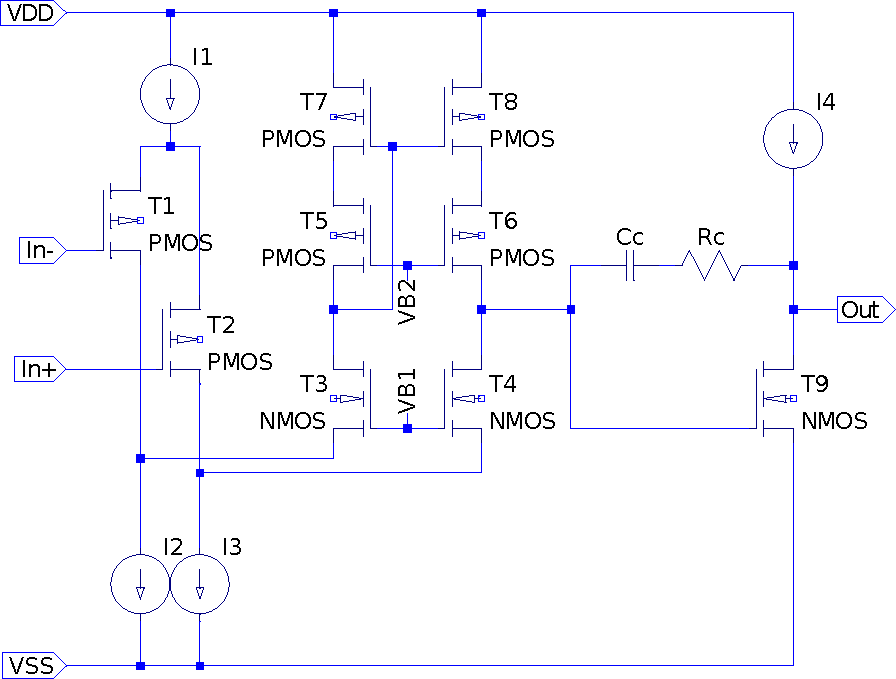
\includegraphics[width=\columnwidth]{schematics/topology.pdf}
  \caption{A schematic of the topology used for the amplifier.}
  \label{fig:topology}
\end{figure}

We next analyzed said amplifier using a simple small signal model, as shown in \Cref{fig:small-signal}. The parameters in the model are given by
\[ G_{m1} = g_{m2} \]
\[ R_{o1} = (r_{o2} g_{m4} r_{o4}) \parallel (r_{o8} g_{m6} r_{o6}) \]
\[ G_{m2} = g_{m9} \]
\[ R_{o2} = r_{o9} \]

\begin{figure}[!htb]
  \centering
  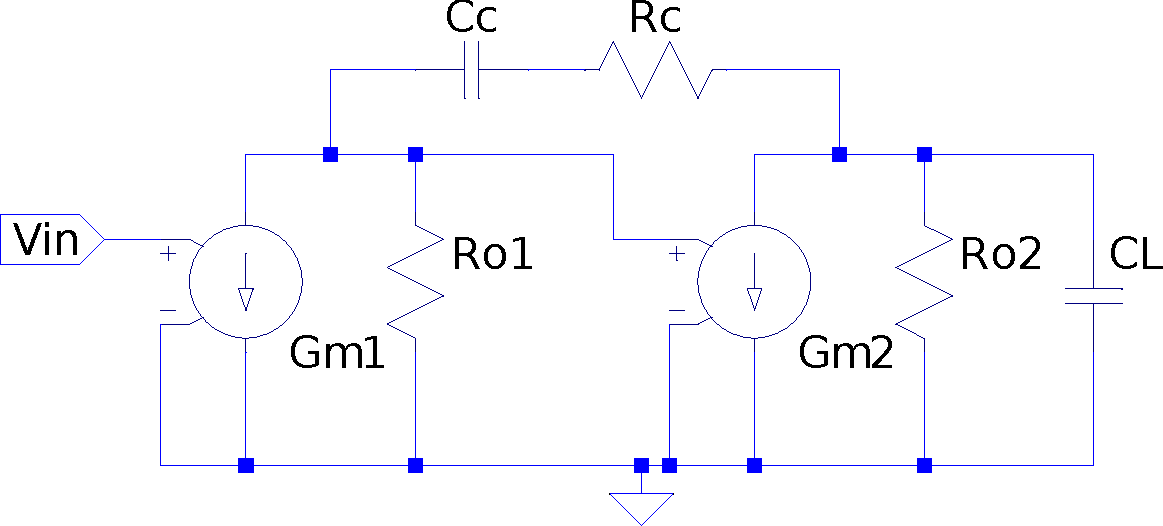
\includegraphics[width=\columnwidth]{schematics/small-signal.pdf}
  \caption{A small signal model of the amplifier in \Cref{fig:topology}.}
  \label{fig:small-signal}
\end{figure}

It can be shown \cite{sedra_microelectronic_2015} that the gain, poles, and zero of the amplifier can be approximated as 
\[ A = G_{m1} R_{o1} G_{m2} R_{o2} \]
\[ f_{p1} = G_{m1} / (2 \pi C_c A) \]
\[ f_{p2} = G_{m2} / (2 \pi C_L)\]
\[ f_{z1} = 1 / (2 \pi C_c (1 / G_{m1} - R_c)) \]

Using $C_L = \SI{0.5}{\pico\farad}$, we obtain $G_{m2} \approx \SI{310}{\micro\ampere\per\volt}$. Taking $C_c = \SI{0.5}{\pico\farad}$ and $A = \SI{5000}{\volt\per\volt}$ for good measure, we also obtain $G_{m1} \approx \SI{160}{\micro\ampere\per\volt}$. Finally, placing the zero at $1.2 f_{p2}$ (in the left half-plane) to smooth out the step response, we obtain $R_c \approx \SI{8.9}{\kilo\ohm}$. Using these parameters as a rough guide, we proceed to performing a first order simulation to find the bias points.

\section{First Order Simulation}

To determine the bias conditions, we replaced current sources $I_1$, $I_2$, and $I_3$ in \Cref{fig:topology} with $\SI{0.2}{\volt}$ voltage sources, meant to represent current mirror transistors operating with $V_{DS} \approx \SI{0.2}{\volt}$. We chose to use a length of $L = \SI{0.4}{\micro\meter}$ for each transistor, several times the minimum length for the process, for adequate analog performance. We then swept the widths $W_1$ and $W_2$ until we obtained $g_{m1} = g_{m2} \approx \SI{160}{\micro\ampere\per\volt}$. With these in hand, we set $V_{B1} = \SI{0.55}{\volt}$ and $V_{B2} = \SI{0.6}{\volt}$ to allow for the proper biasing of transistors $T_3$ to $T_8$. Then, we set $W_5 = W_6 = W_7 = W_8 = \SI{0.4}{\micro\meter}$ and swept $W_3$ and $W_4$ until we obtained a gate voltage for $T_9$ of $V_{G9} \approx \SI{0.5}{\volt}$. Finally, we swept both $I_4$ and $W_9$ until we obtained $V_{Out} \approx \SI{0.5}{\volt}$ and $g_{m9} \approx \SI{310}{\micro\ampere\per\volt}$ to meet our design goals and obtain sufficient output swing. The resulting dimensions are shown in \Cref{tab:dim-first-order}, and the resulting currents are shown in \Cref{tab:bias-first-order}. We note with the current setup, we've only used $\SI{114}{\micro\watt}$ of the power budget, indicating that this criterion is likely to be met with this design.

\begin{table}[!htb]
  \centering
  \caption{Transistor dimensions obtained after a first order simulation of the amplifier.}
  \label{tab:dim-first-order}
  \resizebox{\columnwidth}{!}{\begin{tabular}{|c|c|c|c|c|c|c|c|c|c|}
    \hline
     & T1 & T2 & T3 & T4 & T5 & T6 & T7 & T8 & T9 \\ \hline
    W (\SI{}{\micro\meter}) & 3.5 & 3.5 & 0.65 & 0.65 & 0.4 & 0.4 & 0.4 & 0.4 & 1.4 \\ \hline
    L (\SI{}{\micro\meter}) & 0.4 & 0.4 & 0.4 & 0.4 & 0.4 & 0.4 & 0.4 & 0.4 & 0.4 \\ \hline
  \end{tabular}}
\end{table}

\begin{table}[!htb]
  \centering
  \caption{Bias currents obtained after a first order simulation of the amplifier.}
  \label{tab:bias-first-order}
  \resizebox{0.5\columnwidth}{!}{\begin{tabular}{|c|c|c|c|c|}
    \hline
     & $I_1$ & $I_2$ & $I_3$ & $I_4$ \\ \hline
    I (\SI{}{\micro\ampere}) & 37.5 & 21.3 & 21.3 & 52.0 \\ \hline
  \end{tabular}}
\end{table}

We next performed a pole-zero analysis to see if our design is on the right track to meet the required pole placement. Using our previously calculated values for $C_c$ and $R_c$, we obtained poles at $\SI{5.6}{\kilo\hertz}$ and $\SI{108}{\mega\hertz}$, as well as a zero at $\SI{55}{\mega\hertz}$. These are close enough to the specifications for now, and we will tweak them later when we introduce an actual bias network.

\section{Biasing}

We then replaced the ideal sources with a bias circuit. The completed amplifier is shown in \Cref{fig:amplifier}. Transistors $T_{14}$, $T_{15}$ and resistor $R_b$ generate a reference current that is then mirrored throughout the amplifier to create bias conditions. For the bias network, we only used multiples of a unit size transistor to facilitate matching during layout. Our unit size was $W = \SI{0.4}{\micro\meter}$, $L = \SI{0.4}{\micro\meter}$. With this in mind, we chose $T_{14}$ and $T_{15}$ to be composed of 10 unit size transistors each, and we swept $R_b$ to obtain a bias current of $\SI{10}{\micro\ampere}$. This allowed us to allocate currents in multiples of $\SI{1}{\micro\ampere}$. We thus obtained $R_b = \SI{47}{\kilo\ohm}$.

\begin{figure*}[!htb]
  \centering
  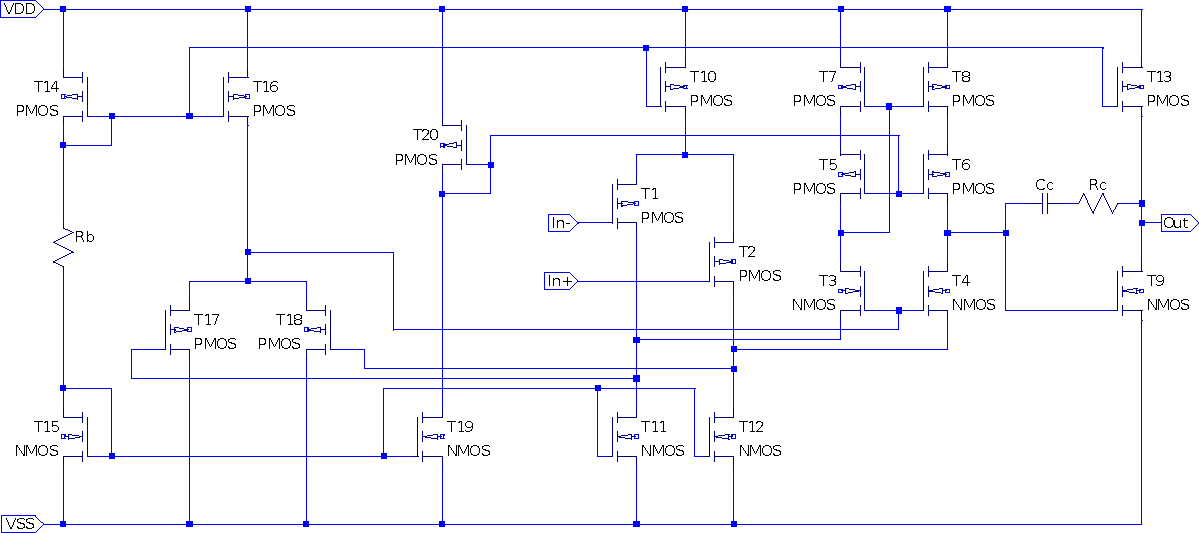
\includegraphics[width=\textwidth]{schematics/amplifier.pdf}
  \caption{A schematic of the complete amplifier with bias network included.}
  \label{fig:amplifier}
\end{figure*}

Transistors $T_{16}$, $T_{17}$, and $T_{18}$ create the bias voltage $V_{B1}$. In order to stabilize the circuit, this voltage is referenced from the sources of $T_3$ and $T_4$. This provides negative feedback which lowers $V_{B1}$ if the drain voltages of $T_{11}$ and $T_{12}$ drop. Transistors $T_{19}$ and $T_{20}$ create the bias voltage $V_{B2}$. Finally, transistors $T_{10}$ to $T_{13}$ generate the bias currents $I_1$ to $I_4$.

We first set the bias network to provide the bias conditions determined in the previous simulation. Then, we corrected for any deviations in order to obtain the proper bias points. One exception was $T_9$. During closed loop testing, we found that this transistor should be set at a lower current in order to maximize the swing. However, this bias condition would lead to triode operation in open loop. This is not actually a problem since we can insert an offset voltage during open loop testing and negative feedback fixes the bias point during closed loop testing. The final transistor dimensions are shown in \Cref{tab:dim-final-1,tab:dim-final-2}.

\begin{table}[!htb]
  \centering
  \caption{Final transistor dimensions (Part 1).}
  \label{tab:dim-final-1}
  \resizebox{\columnwidth}{!}{\begin{tabular}{|c|c|c|c|c|c|c|c|c|c|c|}
    \hline
     & T1 & T2 & T3 & T4 & T5 & T6 & T7 & T8 & T9 & T10 \\ \hline
    W (\SI{}{\micro\meter}) & 3.5 & 3.5 & 0.4 & 0.4 & 2.4 & 2.4 & 0.4 & 0.4 & 1.2 & 13.6 \\ \hline
    L (\SI{}{\micro\meter}) & 0.4 & 0.4 & 0.4 & 0.4 & 0.4 & 0.4 & 0.4 & 0.4 & 0.4 & 0.4 \\ \hline
  \end{tabular}}
\end{table}

\begin{table}[!htb]
  \centering
  \caption{Final transistor dimensions (Part 2).}
  \label{tab:dim-final-2}
  \resizebox{\columnwidth}{!}{\begin{tabular}{|c|c|c|c|c|c|c|c|c|c|c|}
    \hline
     & T11 & T12 & T13 & T14 & T15 & T16 & T17 & T18 & T19 & T20 \\ \hline
    W (\SI{}{\micro\meter}) & 8.0 & 8.0 & 24.0 & 4.0 & 4.0 & 2.8 & 20.0 & 20.0 & 1.6 & 0.4 \\ \hline
    L (\SI{}{\micro\meter}) & 0.4 & 0.4 & 0.4 & 0.4 & 0.4 & 0.4 & 0.4 & 0.4 & 0.4 & 0.4 \\ \hline
  \end{tabular}}
\end{table}

We then reexamined the frequency response of the amplifier. We swept $C_c$ and $R_c$ to obtain the required poles and zeros, and found $C_c = \SI{1}{\pico\farad}$ and $R_c = \SI{3}{\kilo\ohm}$. Using these values, we obtained poles at $\SI{7.4}{\kilo\hertz}$ and $\SI{85}{\mega\hertz}$, and a zero at $\SI{102}{\mega\hertz}$, which meets the specifications.

\section{DC Analysis}

Next, we measured the DC properties of the amplifier using the setup shown in \Cref{fig:open-loop-setup}, where the $\SI{1.2}{\volt}$ power supply has been omitted for clarity.

\begin{figure}[!htb]
  \centering
  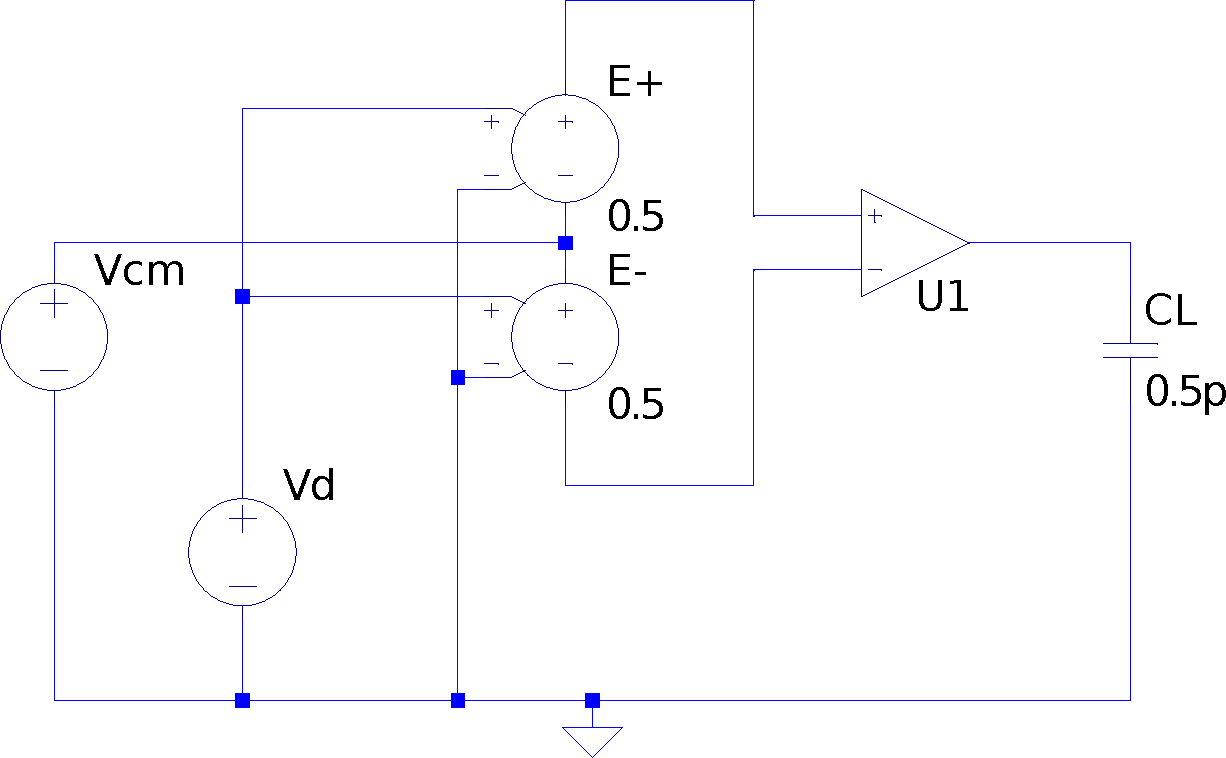
\includegraphics[width=\columnwidth]{schematics/open-loop-setup.pdf}
  \caption{A schematic of the setup used for taking open loop measurements of the amplifier.}
  \label{fig:open-loop-setup}
\end{figure}

We first set the common mode voltage $V_{cm}$ to $\SI{0.5}{\volt}$ and swept the differential mode voltage $V_d$ from $\SI{-5}{\milli\volt}$ to $\SI{5}{\milli\volt}$. The results are shown in \Cref{fig:dc_dm}. From this figure, we can see that the offset voltage is $V_{os} = \SI{335}{\micro\volt}$. We can also see that the output voltage range is $\SI{0.295}{\volt}$ to $\SI{1.03}{\volt}$, corresponding to an input voltage range of $\SI{0.2}{\milli\volt}$ to $\SI{0.6}{\milli\volt}$.

\begin{figure}[!htb]
  \centering
  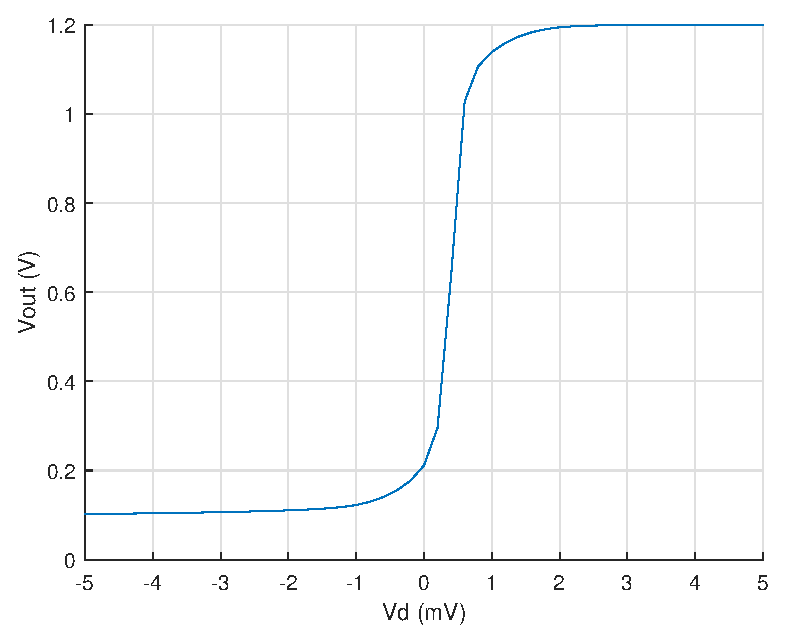
\includegraphics[width=\columnwidth]{figures/dc_dm.eps}
  \caption{DC differential mode transfer characteristic of the amplifier.}
  \label{fig:dc_dm}
\end{figure}

We next measured the common mode transfer characteristic by sweeping $V_{cm}$ over the entire supply range with $V_d = \SI{0}{\volt}$. We also corrected the offset voltage by adding a source between the two input terminals with voltage $V_{os}$. The results are shown in \Cref{fig:dc_cm}. From this figure, we can see that the input common mode voltage can range from $\SI{0}{\volt}$ to about $\SI{1}{\volt}$. This is to be expected from the PMOS input stage, which limits the upper common mode level but allows lower common mode levels beyond even $\SI{0}{\volt}$. However, we do see that there are some non-linearities around $\SI{0.6}{\volt}$, which might produce distortion for large input signals.

\begin{figure}[!htb]
  \centering
  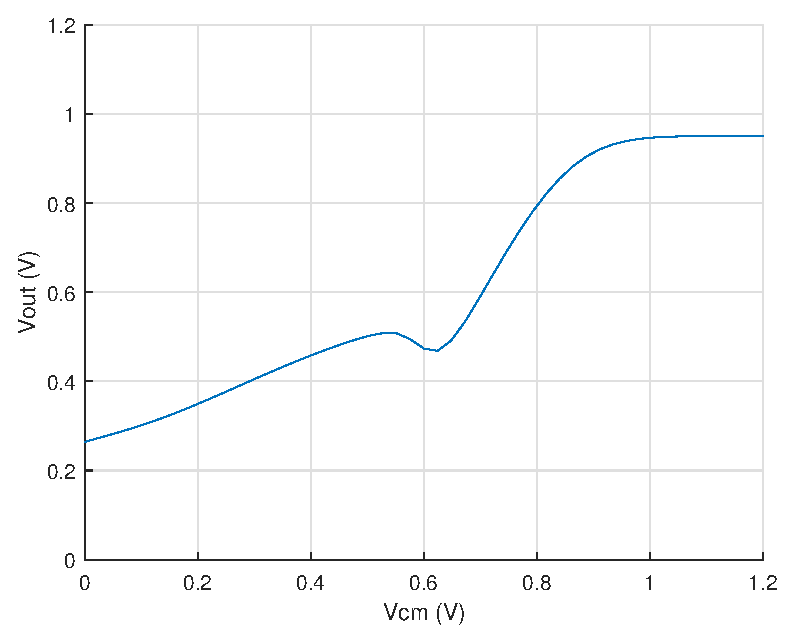
\includegraphics[width=\columnwidth]{figures/dc_cm.eps}
  \caption{DC common mode transfer characteristic of the amplifier.}
  \label{fig:dc_cm}
\end{figure}

We also analyzed the power dissipation of the amplifier. During the DC analysis, the amplifier drew a current of $\SI{125.6}{\micro\ampere}$, which corresponds to a static power dissipation of $\SI{150.7}{\micro\watt}$. Thus, we have met the power dissipation goal of $\SI{200}{\micro\watt}$.

\section{AC Analysis}

We next measured the AC properties of the amplifier using the same setup as in \Cref{fig:open-loop-setup} with the offset corrected. We first measured the differential mode frequency response, and the results are shown in \Cref{fig:ac_dm}. From this figure, we can see that the DC gain is $\SI{65.9}{\deci\bel}$, which meets the specification of DC gain $\ge \SI{60}{\deci\bel}$. A pole-zero analysis showed that the amplifier has its first two poles at $\SI{7.4}{\kilo\hertz}$ and $\SI{85}{\mega\hertz}$, which are both close to the targets of $\SI{10}{\kilo\hertz}$ and $\SI{100}{\mega\hertz}$, respectively. In addition, the first zero is at $\SI{102}{\mega\hertz}$, which is around $1.2$ times the second pole, thus ensuring a smooth frequency response, as we will see later. We can also see that our unity-gain bandwidth is $\SI{14.4}{\mega\hertz}$.

\begin{figure}[!htb]
  \centering
  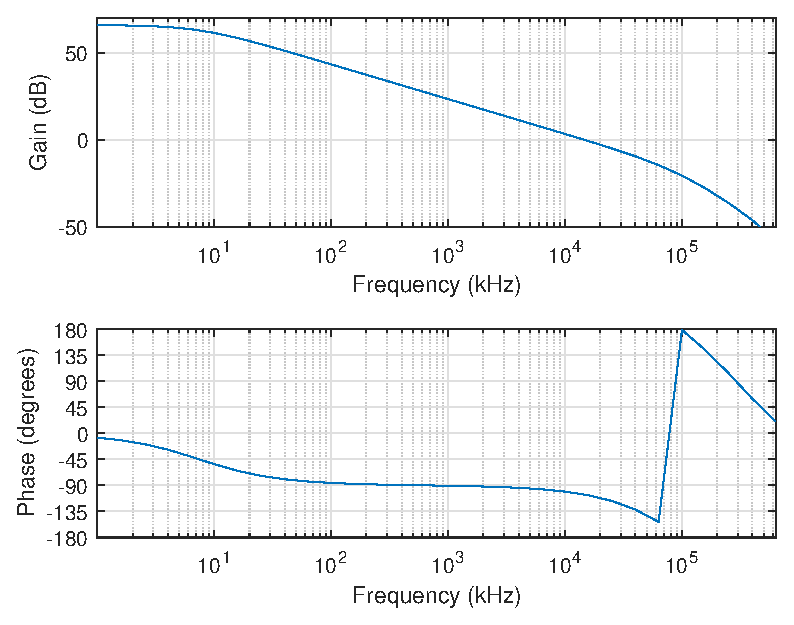
\includegraphics[width=\columnwidth]{figures/ac_dm.eps}
  \caption{AC differential mode frequency response of the amplifier.}
  \label{fig:ac_dm}
\end{figure}

Next, we measured the AC noise of the amplifier using the same setup. Using $V_d$ as our noise source, we obtained the output-referred spectral noise density shown in \Cref{fig:ac_noise}. The noise was measured from $\SI{10}{\hertz}$ to $\SI{1}{\mega\hertz}$, with the RMS value calculated to be $\SI{108}{\milli\volt}$ over this bandwidth. We note that the noise is dominated by flicker noise. In addition, we measured the input-referred spot noise at $\SI{1}{\mega\hertz}$, and found $\SI{40.0}{\nano\volt\per\sqrt{\hertz}}$. This satisfies the upper limit of $\SI{100}{\nano\volt\per\sqrt{\hertz}}$ given in the specifications.

\begin{figure}[!htb]
  \centering
  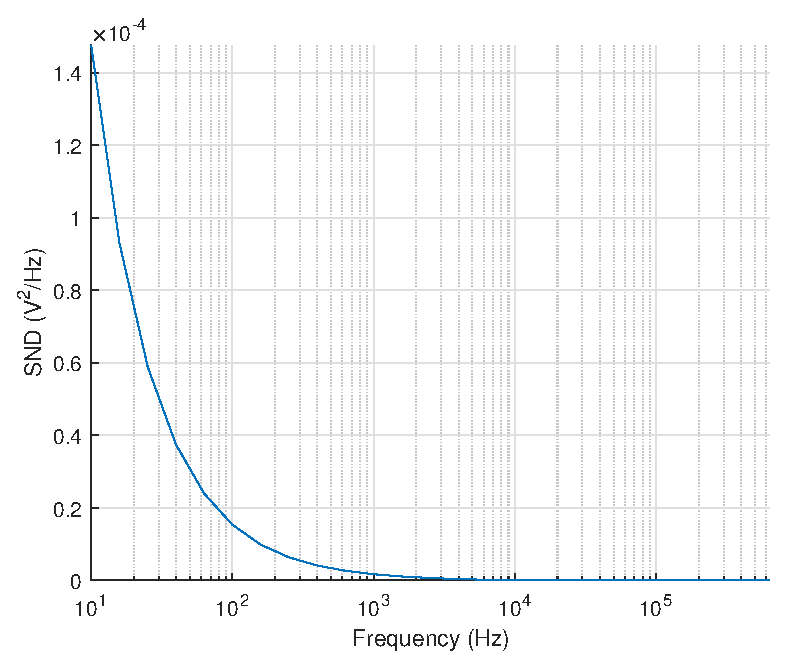
\includegraphics[width=\columnwidth]{figures/ac_noise.eps}
  \caption{Output-referred AC noise of the amplifier.}
  \label{fig:ac_noise}
\end{figure}

\section{Transient Analysis}

We next measured the closed loop transient behaviour of the amplifier using the setup shown in \Cref{fig:closed-loop-setup}, where the $\SI{1.2}{\volt}$ supply has been omitted for clarity.

\begin{figure}[!htb]
  \centering
  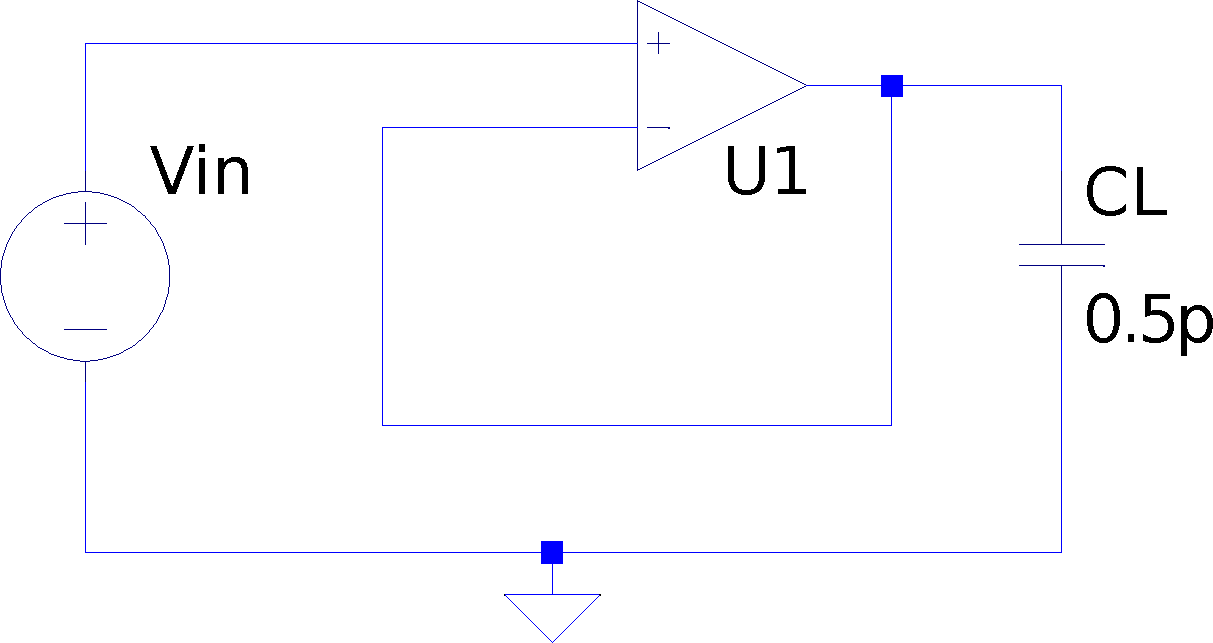
\includegraphics[width=\columnwidth]{schematics/closed-loop-setup.pdf}
  \caption{A schematic of the setup used for taking closed loop measurements of the amplifier.}
  \label{fig:closed-loop-setup}
\end{figure}

First, we input a fast $\SI{100}{\milli\volt}$ pulse to the circuit, starting at a DC bias point of $\SI{0.5}{\volt}$. The resulting output is shown in \Cref{fig:tran_step}. From this graph, we can measure the rise time as $\SI{24.5}{\nano\second}$. Since there is no overshoot, there is no real measure of the settling time.

\begin{figure}[!htb]
  \centering
  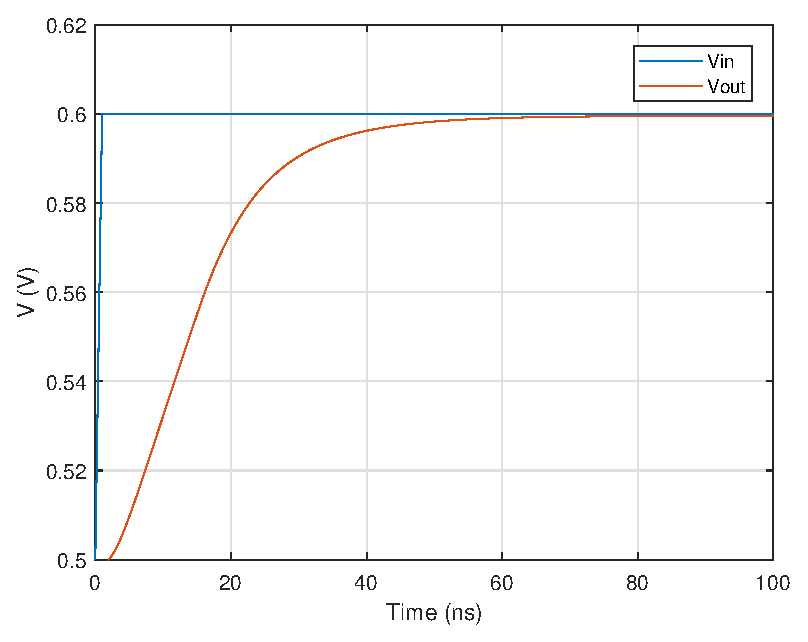
\includegraphics[width=\columnwidth]{figures/tran_step.eps}
  \caption{Transient step response of the amplifier.}
  \label{fig:tran_step}
\end{figure}

Next, we measured the distortion present when we input a $\SI{0.6}{\volt}$ peak-peak sine wave centered around the common mode point of $\SI{0.5}{\volt}$. This corresponds to a swing of half the supply range. The resulting output is shown in \Cref{fig:tran_3m}. From this figure, we can measure the total harmonic distortion as $\SI{0.05}{\percent}$. Thus, we have exceeded the specification of $\SI{0.2}{\percent}$ distortion at a swing equal to half the supply range. Therefore, the amplifier meets all the requirements.

\begin{figure}[!htb]
  \centering
  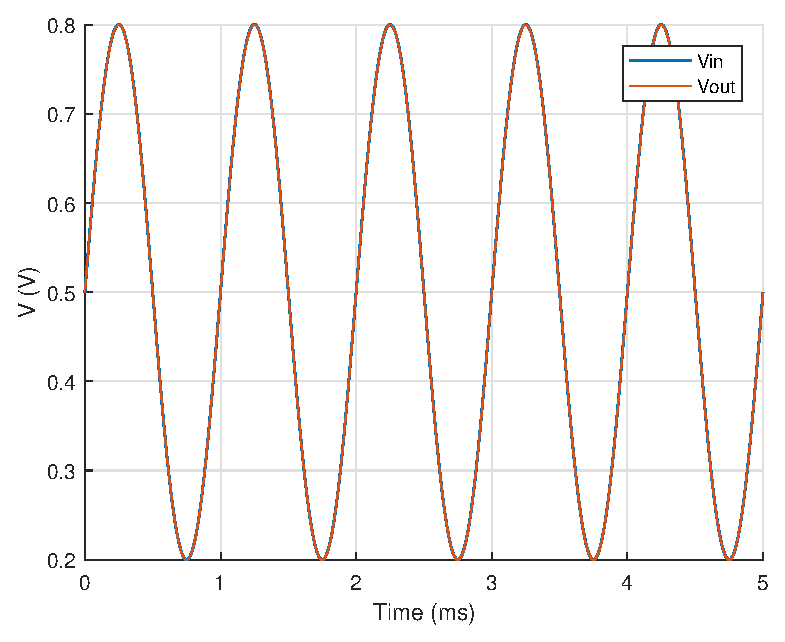
\includegraphics[width=\columnwidth]{figures/tran_3m.eps}
  \caption{Transient response of the amplifier to a $\SI{1}{\kilo\hertz}$, $\SI{300}{\milli\volt}$ amplitude sine wave input.}
  \label{fig:tran_3m}
\end{figure}

Finally, we measured the maximum input/output swing in the unity-gain configuration. To this end, we input a $\SI{1.6}{\volt}$ peak-peak, $\SI{1}{\kilo\hertz}$ sine wave centered around a DC bias point of $\SI{0.5}{\volt}$ and observed the output. The result is shown in \Cref{fig:tran_8m}. This graph shows a maximum input/output swing of $\SI{0.1}{\volt}$ to $\SI{0.92}{\volt}$. We note that the lower limit is given by the output transistor $T_9$ exiting saturation, while the upper limit is given by the input biasing transistor $T_{10}$ exiting saturation, which explains why the swing is greater in the lower limit.

\begin{figure}[!htb]
  \centering
  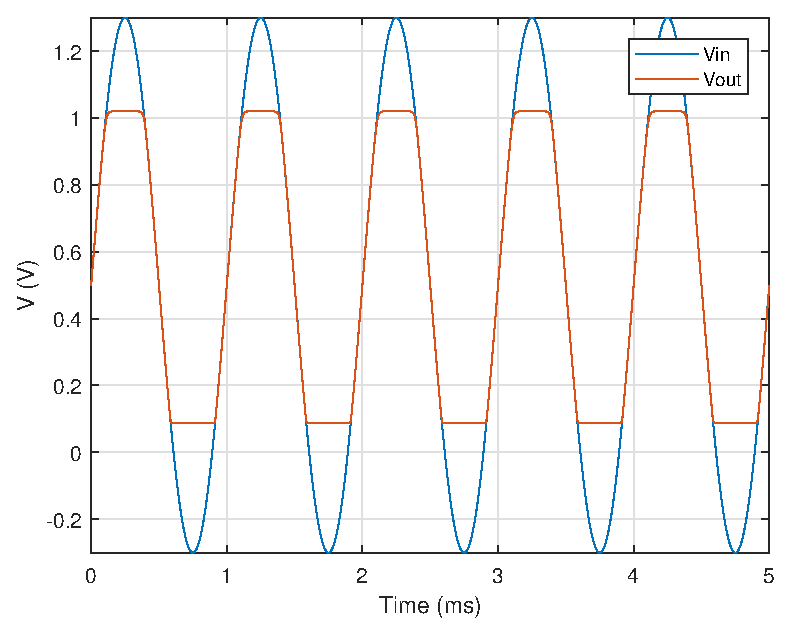
\includegraphics[width=\columnwidth]{figures/tran_8m.eps}
  \caption{Transient response of the amplifier to a large $\SI{1}{\kilo\hertz}$ sine wave input.}
  \label{fig:tran_8m}
\end{figure}

\section{Conclusions}

In conclusion, we designed, simulated, and analyzed an operational amplifier that meets several specifications, including a DC gain greater than $\SI{60}{\deci\bel}$, poles at approximately $\SI{10}{\kilo\hertz}$ and $\SI{100}{\mega\hertz}$, low distortion when swinging at half the supply range, low input-referred noise, and a static power dissipation of less than $\SI{200}{\micro\watt}$.

\bibliographystyle{IEEEtran}
\bibliography{IEEEabrv,references}

\end{document}
